\section{Experiments}

We have implemented and trained our SAMNet model using MI-Prometheus~\cite{kornuta2018accelerating}, a framework based on Pytorch~\cite{paszke2017automatic}. 
We evaluated the model on the COG dataset~\cite{yang2018dataset}, a video reasoning~\cite{mogadala2019trends} dataset developed for the purpose of research on relational and temporal reasoning.
Our experiments were designed to study SAMNet's performance as well as its generalization abilities in different settings.
For this purpose, we used two different variants of the COG dataset (\cref{tab:cog_variants}): an easy one (Canonical) and a Hard version to explore a wide range of difficulties.
The main differences are the number of frames in the input sequence (4 vs. 8) and the maximum number of distractors (i.e., objects not relevant for the answer) per a single frame (1 vs. 10).


\begin{table}[htb]
\caption{Details of the Canonical and Hard variants of the COG dataset}
\centering
\begin{tabular}{lcccccc}
	\toprule
	Variant    &  	number &  	maximum & maximum & size & size & size  \\ 
	& of   & memory & number of & of & of & of  \\
	& frames & duration & distractors & training set & validation set & test set \\
	\midrule
	Canonical & 4 & 3 & 1 & 10000320 & 500016? & 500016 \\	
	Hard  & 8 & 7 & 10 & 10000320 & 500016?  & 500016 \\
	\bottomrule	
\end{tabular}
\label{tab:cog_variants}
\end{table}


%More details on the dataset, its variants and tasks can be found in the Appendix.


%
%We compare our model to the original COG model  ~\cite{yang2018dataset} using their implementation (https://github.com/google/cog) and scores given by the authors. We also use the exact same training parameters detailed in the original paper.
%
%On the other side we trained SAMNet using IBM's Mi-Prometheus~\cite{kornuta2018accelerating}, a framework for research based on Pytorch. We trained all our models using NVIDIA’s GeForce GTX TITAN X GPUs. We trained  SAMNet using 8 reasoning steps SAMCells and a hidden state size of 128. The external memory has 128-bit slots. We trained our model until convergence but we also have set a training time limit of 80 hours.

\subsection{Performance comparison with the COG baseline}

In our experiments we have trained SAMNet using 8 reasoning steps and external memory having 8 address locations, each being a vector of 128 floats.
We have also carried out experiments with different numbers of reasoning steps and memory size, but this goes beyond the scope of this paper.
In here, we have focused on 22 classification tasks and compared our results with the baseline model.
The most important results are highlighted in~\cref{fig:samnet_cog_detailed}, whereas full comparison with all accuracies can be found in the table in the Appendix.

\begin{figure}[htbp]
	\centering
  \begin{subfigure}{\textwidth}
    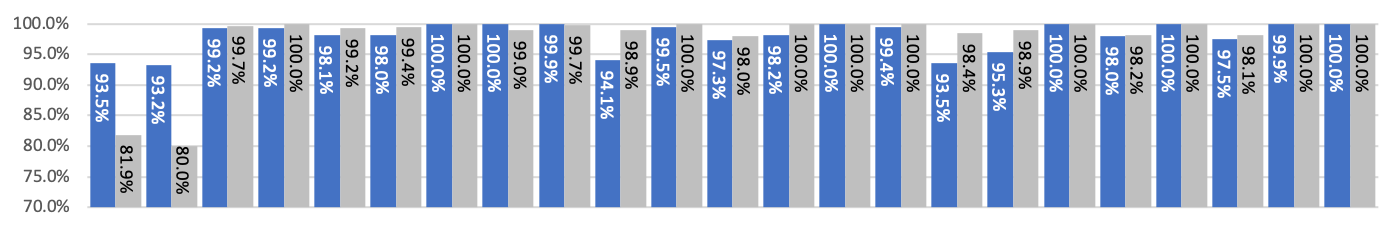
\includegraphics[width=0.99\textwidth]{../results/samnet_cog_orig_canonical_no_labels.png}
  \end{subfigure}%
  \newline
  \begin{subfigure}{\textwidth}
	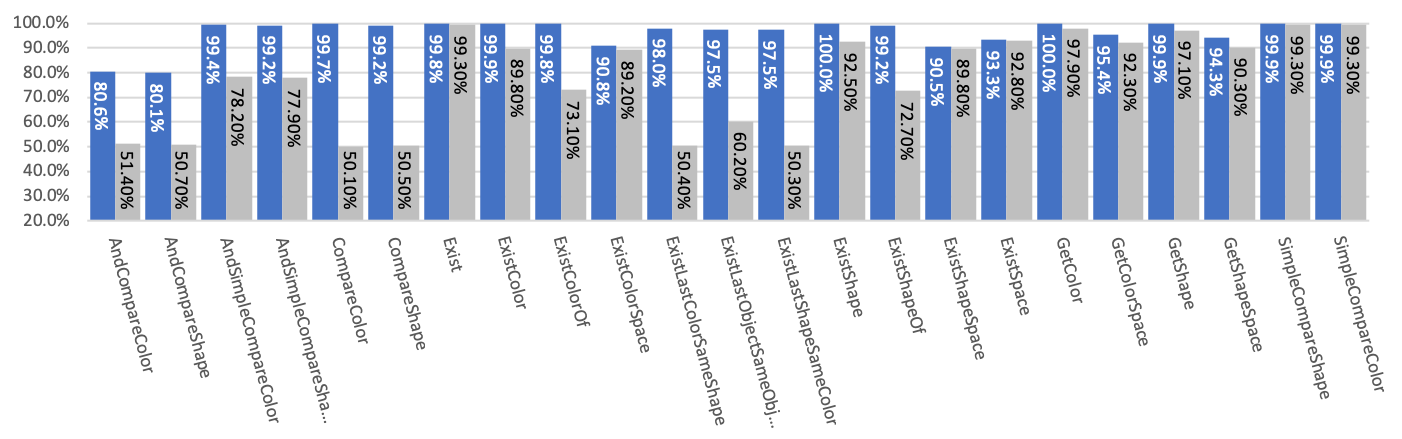
\includegraphics[width=\textwidth]{../results/samnet_cog_orig_hard.png}
  \end{subfigure}%
\caption{Comparison of test set accuracies of SAMNet (blue) with original results achieved by the COG model (gray) on Canonical (top) and Hard (bottom) variants of the COG dataset.}
\label{fig:samnet_cog_detailed}
\end{figure}


For the Canonical variant (top row), we have achieved similar accuracies for the majority of tasks (with the total average accuracy of 98.0\% in comparison of 97.6\% achieved by the COG model), with significant improvements (around 13 points) for \textit{AndCompare} tasks.
As those tasks focus on compositional questions referring to two objects, we hypothesize that our model achieved better accuracy due to the ability to selectively pick and store the relevant objects from the past frames in the memory.
Despite there are some tasks in which our model reached slightly lower accuracies,
% (between 0.2 and 1.8 points)
when comparing performances on the Hard variant, it dominates COG baseline on all tasks, with improvements varying from 0.5 to more than 30 points.


\subsection{Generalization capabilities}

\begin{wrapfigure}{r}{0.5\textwidth}
	\centering
	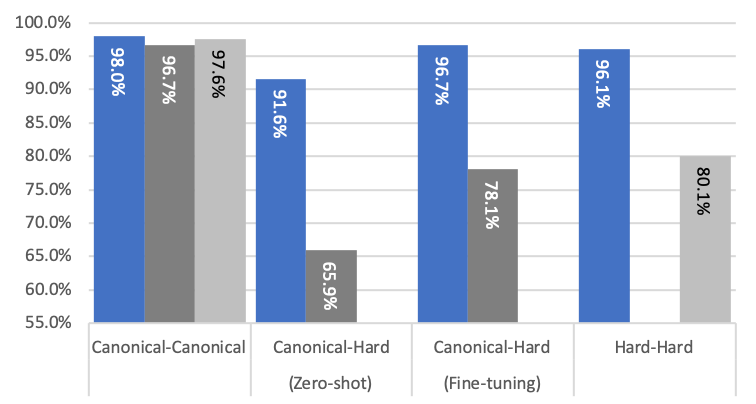
\includegraphics[width=0.5\textwidth]{../results/samnet_cog_overall_transfer.png}
	\caption{Total accuracies of SAMNet (blue) and COG models (light/dark gray) when testing generalization from Canonical to Hard variants of the dataset.}
	\label{fig:samnet_cog_overall_transfer}
\end{wrapfigure}

The goal of the next set of experiments was to test the generalization ability concerning the sequence length and number of distractors.
For that purpose, we have compared the accuracies of both models when trained on the Canonical variant and tested on Hard (\cref{fig:samnet_cog_overall_transfer}).
As the original paper does not include such experiments, we have performed them on our own.  The light gray color indicates the original results, whereas dark gray indicates the accuracies of COG models that we have trained (fine-tuning/testing) using the original code provided by the authors.
For sanity check, in the first column, we report both the best-achieved score and the score reported in the paper when training and testing on Canonical variant, without any fine-tuning.
In a pure \textit{transfer learning} setup (second column), our model shows enormous generalization ability, reaching 91.6\% accuracy on the test set.
We have also tested both models in a setup where the model trained on a Canonical variant underwent additional fine-tuning (for a single epoch) on the Hard variant (third column).
In this case, the SAMNet model also reached much better performance, and, interestingly, achieved better scores from the model trained and tested exclusively on the Hard variant.

%we used the canonical (easy) and hard settings that alter the number of distractors and sequence length.  Since there was no baseline for these tests (train on canonical, test on hard), we ran our own experiments using the COG model provided by the authors.  SAMNet achieves the highest overall scores for all categories of experiments (\cref{fig:samnet_cog_overall_transfer}), especially for the tests run on the hard dataset.  Among the 22 classification tasks, we highlighted the two most difficult tasks that affect the overall score. 
%We argue that the generalization capability of SAMNet is mainly due to the dynamic frame-by-frame processing of the input sequence. 
%The mechanisms introduced in SAMCell learn to operate independently of the total number of frames and allow to generalize to longer video lengths.
%As shown in \cref{fig:samnet_cog_overall_transfer}, when trained on the easy dataset, SAMNet still performs 91.6\% when tested on the hard dataset, whereas COG drops from 97.6\% to 65.9\%   The visualization of the trained SAMNet model (see Appendix) indicates that the model learns the concept of time, helping it to control the flow of information from visual input to the memory.  Therefore, the memory is updated efficiently instead of storing all information across all frames.

\captionsetup[subfigure]{labelformat=empty}
\begin{figure}[htbp]
  \begin{center}
  Question: \textbf{Does color of u now equal the color of the latest circle?}
  \end{center}
  \vskip -0.4cm
  \null\hfill
  \begin{subfigure}{0.25\textwidth}
	\includegraphics[width=0.9\linewidth]{"../img/visualization/experiment_run_20190917_022319/Frame 1"}
	\caption{Frame: \textbf{1}\newline Ground Truth: \textbf{false}}
	\label{fig:frame-1}
  \end{subfigure}%
  \hfill
  \begin{subfigure}{0.25\textwidth}
	\centering
	\includegraphics[width=0.9\linewidth]{"../img/visualization/experiment_run_20190917_022319/Frame 2"}
	\caption{Frame: \textbf{2}\newline Ground Truth: \textbf{false}}
	\label{fig:frame-2}
  \end{subfigure}%
  \hfill
  \begin{subfigure}{0.25\textwidth}
	\centering
	\includegraphics[width=0.9\linewidth]{"../img/visualization/experiment_run_20190917_022319/Frame 3"}
	\caption{Frame: \textbf{3}\newline Ground Truth: \textbf{true}}
	\label{fig:frame-3}
  \end{subfigure}%
  \hfill
  \begin{subfigure}{0.25\textwidth}
	\centering
	\includegraphics[width=0.9\linewidth]{"../img/visualization/experiment_run_20190917_022319/Frame 4"}
	\caption{Frame: \textbf{4}\newline Ground Truth: \textbf{true}}
	\label{fig:frame-4}
  \end{subfigure}%
  \hfill\null
  \newline
  \centering
\caption{A sample from the COG dataset selected for the following analysis.} 
\label{fig:example}  
\end{figure}

\subsection{Analysis of the reasoning strategy}
As a result of training the SAMNet developed a quite complex reasoning strategy.
We will illustrate the key reasoning steps taken by the model on the example presented in \cref{fig:example}.
We have decided to pick the sample from the "AndCompareColor" task, as, despite the clear improvement over the COG baseline model, our SAMNet model seems to still struggle with those type of questions.	

First, let us analyze, independently of SAMNet, what are the key operations that one would need to perform in order to provide the correct answers. 
As the question concerns both the \textbf{now} and \textbf{latest} temporal contexts, in the Frame \textbf{1} one should look for both \textbf{u} and \textbf{circle} objects, look at their colors (different), and provide the answer \textbf{false}.
Next, one should also memorize the \textbf{pink circle} and move to next Frame.
Analogically, in Frame \textbf{2} there are both objects present, both with different colors, so the answer is once again \textbf{false}.
However, from that point we do not care anymore about the \textbf{pink circle} and should remember the \textbf{yellow circle} instead.
This is of utmost importance for the following two frames, as there are no circles present there.
So when analyzing Frames \textbf{3} and \textbf{4} one need to recall the \textbf{yellow circle} from the memory and compare its color with the color of \textbf{u}'s -- as in both cases they are yellow, thus  both answers should be \textbf{true}.

\begin{figure}[!h]
	\centering
	\includegraphics[width=0.95\textwidth]{"../img/visualization/experiment_run_20190917_022319/Frame 2 Step 1"}
	\caption{State of the SAM Cell after 1-st step of reasoning on Frame 2.} 
	\label{fig:frame-2-step-1}
\end{figure}

As full step-by-step analysis (8 reasoning steps for each of 4 frames) would significantly exceed the page limits, we have cherry picked four steps of reasoning performed by our SAMNet model.
Let us start from \textbf{1}-st reasoning step on Frame \textbf{2}, as visualized in \cref{fig:frame-2-step-1} and focus on different aspects of the model.
First, the attention over both the question and image is clearly focusing over the \textbf{u} -- despite we have never trained the system with "word \textbf{u}"-"visual object \textbf{u}" pairs, the SAM Network managed to develop visual grounding on its own.
Second, the time context is clearly focused on \text{Now} -- once again, during the training we have never instructed that the system should pay attention to this (or any other) particular word and the system learned to catch the temporal context on its own (i.e. learned to use the provided mechanisms in the correct way).
Third, as write head is always pointing at "free memory slot", we can notice that there is an object already stored in memory under address 1.
This is the \textbf{pink circle} object memorized during the analysis of the Frame \textbf{1}.
However, we can also notice that the 2nd slot seems to be partially "polluted" by the object from slot 1, which indicates that the write head was not perfectly focused on a single memory address (similarly to the current state).


\begin{figure}[!h]
\centering
  \includegraphics[width=0.95\textwidth]{"../img/visualization/experiment_run_20190917_022319/Frame 2 Step 6"}
\caption{State of the SAM Cell after 6-th step of reasoning on Frame 2.} 
\label{fig:frame-2-step-6}
\end{figure}

Next, let us analyze the \textbf{6}-th reasoning step presented~\cref{fig:frame-2-step-6}.
Here the system clearly focuses its attention on the second object important from the point of view of the question: the \textbf{yellow circle}.
Analogically, the question and visual attention are almost perfectly aligned with the word and object, and, besides, the system  properly caught the time context of the object: \textbf{Latest}.
Additionally, the "Add New" gate is on, the memory address 2 has a different content and write head moved to the next address.
Those are clear indicators that the system has stored the \textbf{yellow circle} in the external memory.
Sadly, also  in here we observe the "pollution" of addresses 3 and 4.

\begin{figure}[!h]
	\centering
	\includegraphics[width=0.95\textwidth]{"../img/visualization/experiment_run_20190917_022319/Frame 4 Step 1"}
	\caption{State of the SAM Cell after 1-st step of reasoning on Frame 4.} 
	\label{fig:frame-4-step-1}
\end{figure}

Let us now fast-forward to analogical reasoning steps in Frame \textbf{6}.
In the \textbf{1}-st reasoning step (\cref{fig:frame-4-step-1}) we can once again observe that  system correctly grounded the visual object \textbf{u} and detected the correct temporal context \textbf{Now}.
Besides that, we can notice that memory content remained more or less unchanged, despite the fact that write head shifted to the next memory address (it also became more soft, pointing at addresses 4 and 5).

\begin{figure}[!h]
	\centering
	\includegraphics[width=0.95\textwidth]{"../img/visualization/experiment_run_20190917_022319/Frame 4 Step 6"}
	\caption{State of the SAM Cell after 6-th step of reasoning on Frame 4.} 
	\label{fig:frame-4-step-6}
\end{figure}

In \textbf{6}-th reasoning step (\cref{fig:frame-4-step-6}) there are several things worth discussing.
First, question attention is pointing at the word \textbf{circle}, but the visual attention is clearly avoiding all the objects. 
This is because there is no circle.
However, as the system properly identified the temporal context as \textbf{Latest}, instead of using the visual object, it uses the object retrieved from the memory -- please notice that the read head, despite not being perfectly crisp, is pointing at addresses 3-5, where it previously stored the \textbf{yellow circle} during the analysis of Frame \textbf{2}.
Moreover, the ``Add New`` gate value is high enough so it once again updates the memory, with void object. 
But please notice that the content of those memory addresses is negligible, and at the end the SAMNet model is still able return the correct prediction.
